%Adaped by Sumesh A K (ak_sumesh@cb.amrita.edu) 2026
%\documentclass[PhD,two side]{ugthesis}
%\documentclass[MS]{ugthesis}
\documentclass[MTech]{ugthesis}
%\documentclass[BTech]{ugthesis}
\usepackage{times}
\usepackage{dashrule}
\usepackage{t1enc}
\usepackage{tikz}
\usepackage{subfigure}
\usepackage{setspace}
\usepackage{geometry}
\usepackage{graphicx}
\usepackage{epstopdf}
\usepackage{lscape}
\usepackage{fancyhdr}
\usepackage{natbib}
\usepackage{hyperref} % hyperlinks for references.
\usepackage{amsmath} % easier math formulae, align, subequations \ldots
\usepackage{amssymb}
\usepackage{wasysym}
\usepackage{titlesec}
\usepackage{textcomp}
\usepackage{pifont}
\usepackage{url}
\usepackage[toc,page]{appendix}
\usetikzlibrary{decorations.pathmorphing}
\usetikzlibrary{shapes,arrows,shadows,patterns,positioning,calc}
\usepackage[printonlyused]{acronym}
\setcounter{MaxMatrixCols}{20}
\captionsetup[figure]{labelfont=bf}
    \appendixpageoff
\renewcommand{\appendixpagename}{APPENDIX} % Changes the title page
\renewcommand{\appendixtocname}{APPENDIX}  % Changes name in TOC
\graphicspath{{figures/}}
\begin{document}
%%%%%%%%%%%%%%%%%%%%%%%%%%%%%%%%%%%%%%%%%%%%%%%%%%%%%%%%%%%%%%%%%%%%%%
% Title page

\title{Coronary Artery Disease Prediction using a Cooperative GA--PSO Hybrid Algorithm and Machine Learning}
\firstauthor{Gokulkannan R M}
\firstauthorregno{[CB.SC.P2CSE25010]}
\guide{Dr. Jeyakumar G.}
\designation{Designation} % TODO: enter the guide's designation
\guidedepartment{Computer Science and Engineering}
\hod{Dr. P. Bagavathi Sivakumar}
\department{COMPUTER SCIENCE AND ENGINEERING}
\date{NOVEMBER 2026}

\maketitle
%%%%%%%%%%%%%%%%%%%%%%%%%%%%%%%%%%%%%%%%%%
\certificate
%\declaration
%%%%%%%%%%%%%%%%%%%%%%%%%%%%%%%%%%%%%%%%%%
\acknowledgements
\normalfont
I would like to express my deep gratitude to our beloved Chancellor Satguru Sri Mata Amritanandamayi Devi for providing a bright academic climate in this university, which has made this entire task appreciable. I would like to thank the management of Amrita Vishwa Vidyapeetham and the entire fraternity of the Department of Computer Science and Engineering, Amrita School of Computing, for providing me with the necessary infrastructure required for the completion of the project.
I wish to record my deep sense of gratitude and profound thanks to my research supervisor Dr. Jeyakumar G., Designation, Department of Computer Science and Engineering, Amrita School of Computing, Amrita Vishwa Vidyapeetham, Coimbatore, for his keen interest, inspiring guidance and constant encouragement with my work during all stages, to bring this thesis into fruition.
I extend my sincere thanks and gratitude to all the members of the review panel, for their timely guidance and suggestions for the improvement of my thesis work.
I would like to extend my sincere thanks to my family and friends for helping and motivating me throughout the course of this project.
Finally, I would like to thank all those who have helped, guided and encouraged me directly or indirectly during the project work.
Above all, I extend my heartfelt salutations to my beloved parents and Almighty, for their blessings and grace, for the successful completion of this thesis.
\vskip 25pt
\noindent
Name: Gokulkannan R M\\
Roll No: CB.SC.P2CSE25010\\
Signature:\\

%%%%%%%%%%%%%%%%%%%%%%%%%%%%%%%%%%%%%%%%%%
\abstract
\begin{onehalfspacing}
\normalfont
{\noindent
Predicting coronary artery disease (CAD) from routine clinical attributes depends heavily on which attributes a model uses and how its hyperparameters are set. Most evolutionary hybrids make these two choices one after the other, with no feedback. This thesis designs and evaluates a cooperative alternative in which a Genetic Algorithm (GA) searches binary feature masks and Particle Swarm Optimization (PSO) tunes the classifier, and the two exchange their best solutions in every round under a shared, leakage-free cross-validated F1 objective. On the Cleveland dataset (303 patients, 13 attributes), a full cooperative run for a Support Vector Machine (SVM) selected 8 attributes and reached an out-of-fold accuracy of 0.865 and a Matthews correlation coefficient (MCC) of 0.727. Because this estimate is optimistic, the main experiment uses nested cross-validation (5 outer folds, 3 seeds) to compare the cooperative scheme with baseline, GA-only, PSO-only and sequential GA--PSO variants. The cooperation improved the inner search in every round, but on unseen patients the cooperative SVM (accuracy 0.811, MCC 0.622) was no better than the sequential and GA-only variants and was significantly worse than PSO tuning on all attributes (accuracy 0.838, MCC 0.676; Wilcoxon $p<0.01$). The result held without the feature penalty and with repeated inner folds. Selected subsets were unstable, showing that wrapper feature selection overfits at this sample size. An audit also shows that all 270 Statlog records are contained in Cleveland. The thesis concludes that hybrid feature-selection schemes for small CAD datasets must be judged by nested, ablated evaluation.
}
\end{onehalfspacing}

\pagebreak
%%%%%%%%%%%%%%%%%%%%%%%%%%%%%%%%%%%%%%%%%%%%%%%%%%%%%%%%%%%%%%%%%
% Table of contents etc.

\begin{singlespace}
\tableofcontents
\thispagestyle{empty}

\listoftables
\addcontentsline{toc}{chapter}{List of Tables}
\listoffigures
\addcontentsline{toc}{chapter}{List of Figures}
\end{singlespace}

%%%%%%%%%%%%%%%%%%%%%%%%%%%%%%%%%%%%%%%%%%%%%%%%%%%%%%%%%%%%%%%%%%%%%%
\abbreviations
\begin{acronym}[XGBoost]
\acro{ANN}{Artificial Neural Network}
\acro{AP}{Average Precision}
\acro{AUC}{Area Under the ROC Curve}
\acro{CAD}{Coronary Artery Disease}
\acro{CV}{Cross-Validation}
\acro{CVD}{Cardiovascular Disease}
\acro{DEAP}{Distributed Evolutionary Algorithms in Python}
\acro{DL}{Deep Learning}
\acro{DT}{Decision Tree}
\acro{EA}{Evolutionary Algorithm}
\acro{ECG}{Electrocardiogram}
\acro{EO}{Evolutionary Optimization}
\acro{FN}{False Negative}
\acro{FP}{False Positive}
\acro{GA}{Genetic Algorithm}
\acro{MCC}{Matthews Correlation Coefficient}
\acro{ML}{Machine Learning}
\acro{MLP}{Multilayer Perceptron}
\acro{NN}{Neural Network}
\acro{PR}{Precision--Recall}
\acro{PSO}{Particle Swarm Optimization}
\acro{RBF}{Radial Basis Function}
\acro{RF}{Random Forest}
\acro{ROC}{Receiver Operating Characteristic}
\acro{SDG}{Sustainable Development Goal}
\acro{SHAP}{SHapley Additive exPlanations}
\acro{SMOTE}{Synthetic Minority Over-sampling Technique}
\acro{SVM}{Support Vector Machine}
\acro{TN}{True Negative}
\acro{TP}{True Positive}
\acro{UCI}{University of California, Irvine}
\acro{WHO}{World Health Organization}
\acro{XGBoost}{eXtreme Gradient Boosting}
\end{acronym}

\pagebreak

%%%%%%%%%%%%%%%%%%%%%%%%%%%%%%%%%%%%%%%%%%%%%%%%%%%%%%%%%%%%%%%%%%%%%%
\chapter*{\centerline{List of Symbols}}
\addcontentsline{toc}{chapter}{List of Symbols}
\begin{doublespace}
\begin{tabbing}
xxxxxxxxxxxxxx \= xxxxxxxxxxxxxxxxxxxxxxxxxxxxxxxxxxxxxxxxxxxxxxxx \kill
\textbf{$c_1$, $c_2$}   \> Cognitive and social acceleration coefficients of PSO \\
\textbf{$C$}            \> SVM regularisation parameter \\
\textbf{$d$}            \> Number of candidate features (13) \\
\textbf{$F(\mathbf{m},\boldsymbol{\theta})$} \> Penalised fitness of mask $\mathbf{m}$ with hyperparameters $\boldsymbol{\theta}$ \\
\textbf{$\gamma$}       \> RBF kernel width parameter of the SVM \\
\textbf{$K$}            \> Number of cross-validation folds \\
\textbf{$\lambda$}      \> Per-feature penalty coefficient \\
\textbf{$\mathbf{m}$}   \> Binary feature mask, $\mathbf{m}\in\{0,1\}^d$ \\
\textbf{$N_g$, $N_p$}   \> GA population size, PSO swarm size \\
\textbf{$p_c$, $p_m$}   \> GA crossover and mutation probabilities \\
\textbf{$r_1$, $r_2$}   \> Uniform random numbers in $[0,1]$ \\
\textbf{$R$}            \> Number of cooperative rounds \\
\textbf{$\boldsymbol{\theta}$} \> Classifier hyperparameter vector \\
\textbf{$\mathbf{v}_i$, $\mathbf{x}_i$} \> Velocity and position of particle $i$ \\
\textbf{$w$}            \> PSO inertia weight \\
\end{tabbing}
\end{doublespace}
\pagebreak
\clearpage
\pagenumbering{arabic}

%%%%%%%%%%%%%%%%%%%%%%%%%%%%%%%%%%%%%%%%%%%%%%%%%%
\chapter{Introduction}
\label{chap:intro}

\ac{CVD} is the largest single cause of death in the world. The \ac{WHO} attributes about 17.9 million deaths a year to it, roughly a third of all deaths, and a large share of these occur in low- and middle-income countries where specialist cardiac care is scarce \citep{who2021cvd}. A confirmed diagnosis of \ac{CAD} normally rests on angiography, stress imaging or a cardiologist's reading of an exercise \ac{ECG}. All of these are costly, need trained staff and are not available at every point of care. There is therefore practical value in a screening aid that estimates the likelihood of disease from attributes that a general clinic can record cheaply: age, sex, chest-pain history, resting blood pressure, cholesterol and a handful of exercise-test readings.

Data-driven classifiers fit this role well. \ac{SVM}s, \ac{RF}s, gradient-boosted trees and small \ac{NN}s have been applied to the \ac{UCI} heart disease collections for over three decades, starting with the probabilistic model of \citet{detrano1989}. Two difficulties keep recurring. The first is that these datasets are small, a few hundred patients at most, so irrelevant or redundant attributes cost more than they would in a large dataset: every extra input gives the model one more way to fit noise. The second is that classifier behaviour is sensitive to hyperparameters. An RBF-kernel SVM with a poorly chosen $C$ and $\gamma$ can lose several points of accuracy compared with a well-tuned one on the same inputs. Feature selection and hyperparameter tuning are thus the two levers with the most influence on the final result.

Combining the two optimizers is not new. What is less settled is \emph{how} to combine them. In the heart disease studies surveyed in Chapter~\ref{chap:lit}, the usual pattern is a pipeline: one stage chooses features, another tunes the model, and each stage treats the other's output as fixed. The best feature subset for a default-parameter SVM need not be the best subset for a tuned one, and the reverse also holds. This thesis examines a cooperative alternative, in which the two searches inform each other repeatedly while they run.

\section{Problem Definition}
\label{sec:problem}
Let $\mathbf{X}\in\mathbb{R}^{n\times d}$ hold $n$ patient records with $d=13$ clinical attributes and let $\mathbf{y}\in\{0,1\}^n$ mark absence or presence of heart disease. For a binary mask $\mathbf{m}\in\{0,1\}^d$ and a hyperparameter vector $\boldsymbol{\theta}$ for a chosen classifier, define $F(\mathbf{m},\boldsymbol{\theta})$ as the classifier's cross-validated F1 score on the columns selected by $\mathbf{m}$, reduced by a small penalty proportional to $\|\mathbf{m}\|_1$. The task is to find
\begin{equation}
(\mathbf{m}^{*},\boldsymbol{\theta}^{*}) = \arg\max_{\mathbf{m},\,\boldsymbol{\theta}} \; F(\mathbf{m},\boldsymbol{\theta}),
\qquad \|\mathbf{m}\|_1 \ge 2,
\label{eq:problem}
\end{equation}
and then to estimate, without bias, how well the resulting model would perform on new patients.

The problem is mixed (discrete $\mathbf{m}$, continuous $\boldsymbol{\theta}$) and coupled, because the best $\mathbf{m}$ depends on $\boldsymbol{\theta}$ and vice versa, so solving it in two isolated stages generally stops short of a joint optimum. The research question of this thesis is whether repeated, scheduled exchange between a GA over $\mathbf{m}$ and a PSO over $\boldsymbol{\theta}$ finds better joint configurations than one-pass pipelines, at an acceptable computational cost.

\section{What This Work Does Differently}
\label{sec:novelty}
Earlier work has already combined evolutionary optimizers with classifiers for heart disease. This thesis differs from it in four ways.
\begin{enumerate}
\item \textbf{Two optimizers, each on the part it suits, with feedback in both directions.} Single-optimizer joint methods \citep{huang2006gasvm,lin2008psosvm,abdar2019n2genetic} put the mask and the parameters into one vector for one algorithm. Pipeline methods \citep{cao2025dlpso,warsi2024gasvm} run feature selection and then tuning, with nothing passed back. Here a binary GA searches the masks and a real-valued PSO searches the parameters. After every round each one passes its best solution to the other, following the cooperative co-evolution model \citep{potter1994cc,ma2019ccsurvey}.
\item \textbf{A test of whether the cooperation itself helps.} The cooperative scheme is compared with GA-only, PSO-only and one-pass sequential GA$\rightarrow$PSO variants under the same fitness-evaluation budget and the same outer folds, with a paired statistical test. Most hybrid studies compare only against untuned models, so they cannot show which part of the hybrid produced the gain.
\item \textbf{Leakage-free, nested evaluation.} Scaling is fitted inside every training fold, and the whole GA--PSO search is repeated inside each outer training fold. The reported scores therefore come from patients the search never saw.
\item \textbf{An audit of the datasets.} The thesis shows that the Statlog heart dataset is a subset of Cleveland. Studies that treat the two as independent, or that pool them, can overstate their accuracy.
\end{enumerate}

\section{Objectives}
\label{sec:objectives}
\begin{enumerate}
\item[O1] Build a reproducible data pipeline and a set of untuned baseline classifiers (SVM, RF, MLP) for the Cleveland and Statlog heart disease datasets, with scaling fitted only on training data.
\item[O2] Design and implement a cooperative GA--PSO optimizer in which a GA selects feature subsets and PSO tunes classifier hyperparameters, exchanging their best solutions every round.
\item[O3] Evaluate the cooperative optimizer for SVM, RF and XGBoost using cross-validated accuracy, F1, \ac{AUC} and \ac{MCC}, and record its convergence and computational cost.
\item[O4] Compare the cooperative design against baseline, GA-only, PSO-only and sequential GA$\rightarrow$PSO variants under a common, leakage-free nested cross-validation protocol, with a paired statistical test.
\item[O5] Audit the benchmark datasets for overlap, and identify which attributes are selected consistently.
\end{enumerate}
Objectives O1, O2, O4 and O5 are complete. O3 is complete for the SVM. The random forest run is partial and XGBoost was not run (Section~\ref{sec:limits}).

\section{Relation to Sustainable Development Goals}
The work relates most directly to \ac{SDG}~3 (Good Health and Well-Being), in particular Target~3.4 on reducing premature mortality from non-communicable disease. Feature selection is the methodological link: a model that needs eight attributes instead of thirteen asks less of the clinic that runs it. Because the method also contributes a general-purpose cooperative optimizer, it is relevant to SDG~9 (Target~9.5, research capability). Classical models that run on ordinary hardware, together with explanations, keep deployment within reach of resource-limited settings, which supports the equity aim of SDG~10.

\section{Organisation of the Thesis}
Chapter~\ref{chap:lit} reviews soft computing in medicine and the specific GA- and PSO-based studies on heart disease, and derives the research gap. Chapter~\ref{chap:proposed} describes the datasets, the preprocessing, the baselines and the cooperative GA--PSO algorithm in detail. Chapter~\ref{chap:results} explains the implementation and reports the baseline results, the cooperative results and the nested cross-validation ablation, together with their limitations. Chapter~\ref{chap:conclusion} summarises the findings and sets out future extensions.

%------------------------------------------------------------------------------------------------%
\chapter{Literature Survey}
\label{chap:lit}

This chapter reviews the two optimizers, earlier methods that select features and tune parameters together, and journal and conference studies that apply evolutionary or swarm methods to CAD and heart disease. It ends with the research gap.

\section{Soft Computing in Biomedical Data Analysis}
Soft computing methods, including neural networks, fuzzy systems, evolutionary computation and swarm intelligence, are widely used for biomedical data. Surveys report steady growth in hybrids that combine them \citep{yardimci2009medicine,houssein2023softcomputing}. They also note that the way the components are joined matters as much as which components are chosen, and that evaluation practice is uneven \citep{xie2014emg}.

\section{Background on the Optimizers}
\subsection{Genetic Algorithm}
A GA keeps a population of candidate solutions encoded as chromosomes \citep{holland1975,goldberg1989}. Each generation, parents are chosen with a bias toward higher fitness, recombined by crossover and perturbed by mutation. For feature selection, the chromosome is simply a bit string of length $d$ in which bit $j$ indicates whether feature $j$ is used. This makes GAs one of the most widely used wrapper methods for feature selection \citep{xue2016fssurvey}. Their strength is global exploration of a discrete space. Their weakness is slow fine-tuning of continuous quantities. \citet{slowik2020ea} give a recent overview of GA variants and engineering applications.

\subsection{Particle Swarm Optimization}
PSO \citep{kennedy1995pso} moves a swarm of particles through a continuous space. Each particle $i$ has a position $\mathbf{x}_i$ and velocity $\mathbf{v}_i$ and remembers its personal best $\mathbf{p}_i$, while the swarm tracks the global best $\mathbf{g}$. With the inertia weight introduced by \citet{shi1998inertia}, the update is
\begin{align}
\mathbf{v}_i^{t+1} &= w\,\mathbf{v}_i^{t} + c_1 r_1 (\mathbf{p}_i - \mathbf{x}_i^{t}) + c_2 r_2 (\mathbf{g} - \mathbf{x}_i^{t}), \label{eq:psov}\\
\mathbf{x}_i^{t+1} &= \mathbf{x}_i^{t} + \mathbf{v}_i^{t+1}. \label{eq:psox}
\end{align}
PSO has few parameters, converges quickly and handles continuous hyperparameters naturally. Its known weakness is premature convergence when the swarm collapses onto one region.

\subsection{Joint feature selection and parameter tuning}
Searching the feature subset and the classifier parameters together is an established idea, and the present work builds on it. \citet{huang2006gasvm} encoded the SVM parameters $C$ and $\gamma$ and a feature mask in one binary GA chromosome and reported higher accuracy with fewer inputs than grid search. \citet{lin2008psosvm} did the same with a single PSO swarm. In both designs one optimizer handles a mixed discrete--continuous vector: the GA has to treat continuous parameters as bit strings, and the PSO has to threshold real numbers to obtain a mask. Each operator is therefore applied to a part of the problem it does not suit. Survey work on evolutionary and swarm feature selection \citep{xue2016fssurvey,nguyen2020sifs} identifies representation as the main design choice in these methods. The design studied here separates the two parts and gives each its natural optimizer, a binary GA for the mask and a real-valued PSO for the parameters, coupled through cooperative exchange.

\subsection{Hybrids of GA and PSO}
Since the two methods have complementary strengths, hybrids appeared early. \citet{juang2004gapso} combined GA and PSO operators inside one population to design recurrent networks. Cooperative coevolution \citep{potter1994cc} offers a different template: the solution is split into parts, each part is evolved by its own population, and each part is evaluated together with the current best representatives of the others. \citet{ma2019ccsurvey} survey the cooperative co-evolution literature and identify problem decomposition, the choice of collaborators and the allocation of computation between sub-populations as its central design questions. The design in this thesis follows that cooperative template. The feature mask and the hyperparameter vector are the two parts, and each has its own optimizer. By the no-free-lunch theorem \citep{wolpert1997nfl}, any benefit has to be shown empirically.

\section{Evolutionary and Swarm Methods for Coronary Artery Disease}
\citet{alizadehsani2019review} review machine-learning studies of \ac{CAD} diagnosis published between 1992 and 2019. They conclude that the reported results are hard to compare, because the studies differ in dataset, sample size, features, metrics and validation method. Several journal studies have used evolutionary or swarm optimizers for CAD in particular. \citet{arabasadi2017nnga} used a GA to choose the initial weights of a neural network on the Z-Alizadeh Sani dataset and reported 93.85\% accuracy, about ten points better than the network trained from random initial weights. \citet{abdar2019n2genetic} proposed N2Genetic-nuSVM, which joins 10-fold cross-validation with GA or PSO to select features and tune an SVM at once. It reached 93.08\% accuracy on the same data. \citet{shahid2020psoemnn} trained an emotional neural network with PSO for CAD diagnosis and found it better than a PSO-tuned neuro-fuzzy system. \citet{velusamy2021ensemble} combined feature-subset selection with a heterogeneous ensemble for CAD.

Hybrid models are also common in general heart disease prediction. \citet{mohan2019hrflm} combined a random forest with a linear model (HRFLM) on Cleveland and reported 88.7\% accuracy. \citet{ghosh2021relief} merged the Cleveland, Hungarian, Swiss, Long Beach VA and Statlog files, used Relief and LASSO for feature selection, and reported up to 99.05\% accuracy. Section~\ref{sec:overlap} shows that every Statlog record already appears in Cleveland. A pooled file of this kind therefore contains duplicated patients, and if copies of one patient land in both the training and test parts, the reported accuracy can be inflated. This is one concrete reason for the large spread of reported figures.

\section{GA- and PSO-based Heart Disease Prediction}
Table~\ref{tab:lit} summarises ten further studies that informed this work. They were identified at the start of the project, and their bibliographic details were checked against the publishers' records. Most of them are conference papers or book chapters, so they are used here to show current practice. The journal studies above provide the main methodological comparison.

In these studies the optimizer is used for a single stage, either feature selection or tuning, or several optimizers are compared rather than combined. The closest design is that of \citet{cao2025dlpso}, who filter features and then tune XGBoost with an improved PSO, again in two consecutive stages with no feedback. Accuracies of 92--98\% are reported without external validation \citep{majumder2025psodt,nagavelli2024pso}.

\begin{table}[htpb]
\small
\renewcommand{\arraystretch}{1.3}
\caption{Summary of GA/PSO-based heart disease prediction studies}
\label{tab:lit}
\begin{tabular}{|p{2.6cm}|p{2.4cm}|p{2.2cm}|p{3.2cm}|p{3.4cm}|}
\hline
\textbf{Study} & \textbf{Optimizer} & \textbf{Model} & \textbf{Reported outcome} & \textbf{Limitation for this work} \\ \hline
\citet{warsi2024gasvm} & GA (features) & SVM & Improved over untuned SVM & One optimizer, one dataset \\ \hline
\citet{kavitha2021hybrid} & None & DT + RF ensemble & 88.7\% accuracy & No optimization stage \\ \hline
\citet{effective2021gasvm} & GA & SVM & Better than plain SVM & Single preparatory stage \\ \hline
\citet{kanchanamala2023spark} & Hybrid metaheuristic & Deep CNN (Spark) & Scalable DL detection & High cost, low interpretability \\ \hline
\citet{zhang2024xgga} & GA, SMA, GAO (compared) & XGBoost and others & 0.972 accuracy (XGGA) & Optimizers not combined \\ \hline
\citet{majumder2025psodt} & PSO & Decision tree & 86.38\% $\rightarrow$ 92.38\% & One optimizer, one dataset \\ \hline
\citet{reddy2025psonn} & PSO & Neural network & Beats other tuned models & Optimizers run in isolation \\ \hline
\citet{nagavelli2024pso} & PSO (features) & SVM, RF, NB, LR & 98\% accuracy & No external test; overfitting risk \\ \hline
\citet{cao2025dlpso} & Filter + improved PSO & XGBoost & Gains over plain XGBoost & Sequential stages, no feedback \\ \hline
\citet{wadhawan2026gavspso} & GA vs.\ PSO & Several & Comparative study & Never combines GA and PSO \\ \hline
\end{tabular}
\end{table}

\section{Findings and Research Gap}
\label{sec:gap}
Three observations emerge from the survey.

First, among the studies that use both a feature-selection step and a tuning step, the two steps are run in sequence with no return path. The feature subset is chosen under one model configuration and then frozen while the configuration changes. This is the structural gap that motivates the cooperative design.

Second, the reported accuracies (88.7\%, 92.38\%, 97.2\%, 98\%) come from different datasets, different splits and different protocols, and are not comparable to one another. Where the feature subset or hyperparameters are chosen on the same folds that are then used to report performance, the estimate is biased upward. This effect is well documented \citep{varma2006bias,cawley2010overfitting}, but rarely addressed in this literature. A related problem, discussed in Chapter~\ref{chap:results}, is that two of the ``independent'' UCI heart datasets overlap heavily.

%------------------------------------------------------------------------------------------------%
\chapter{Proposed Work}
\label{chap:proposed}

This chapter describes the overall architecture, the datasets and preprocessing, the baseline models, and the cooperative GA--PSO algorithm with its fitness function and evaluation protocol.

\section{System Architecture}
Figure~\ref{fig:arch} shows the pipeline. Raw CSV files are loaded and checked, numeric gaps (none in the current data) are filled with column medians, and the target is binarised. Two paths then diverge. The baseline path holds out a stratified 20\% test split and trains untuned classifiers. The cooperative path runs the GA--PSO loop over the full dataset with internal 10-fold cross-validation, then passes the best mask and hyperparameters to the evaluation module, which produces metrics and plots.

\begin{figure}[htpb]
\centering
\tikzstyle{block} = [rectangle, line width=0.75pt, draw, text width=30mm, text centered, minimum height=10mm, font=\footnotesize\bfseries]
\tikzstyle{line} = [draw, line width=0.75pt, -latex']
\begin{tikzpicture}[node distance=8mm and 10mm]
\node [block] (data) {Raw CSV (Cleveland, Statlog)};
\node [block, below=of data] (prep) {Validation, median imputation, target binarisation};
\node [block, below left=of prep, xshift=8mm] (base) {Stratified 80/20 split; scaler fit on train};
\node [block, below=of base] (bm) {Untuned SVM, RF, MLP};
\node [block, below=of bm] (bres) {Hold-out metrics + 5-fold CV accuracy};
\node [block, below right=of prep, xshift=-8mm] (coop) {Cooperative GA--PSO (10-fold CV fitness)};
\node [block, below=of coop] (best) {Best mask $\mathbf{m}^*$ + hyperparameters $\boldsymbol{\theta}^*$};
\node [block, below=of best] (eval) {Evaluation: metrics, ROC/PR, convergence};
\path [line] (data) -- (prep);
\path [line] (prep) -| (base);
\path [line] (prep) -| (coop);
\path [line] (base) -- (bm);
\path [line] (bm) -- (bres);
\path [line] (coop) -- (best);
\path [line] (best) -- (eval);
\end{tikzpicture}
\caption{Overall pipeline of the proposed system}
\label{fig:arch}
\end{figure}

\section{Datasets for the Study and Platform}
\subsection{Datasets}
\textbf{Cleveland.} The Cleveland Clinic subset of the UCI heart disease collection \citep{detrano1989,uci_heart} is the standard benchmark for this task. The version used here contains 303 patients and the 13 attributes listed in Table~\ref{tab:features}, with no missing values. The original target (0--4) is binarised into absence (0, 164 patients) and presence (1, 139 patients) of disease, so the positive class makes up 45.9\% of the data. The classes are therefore close to balanced.

\textbf{Statlog.} The Statlog (Heart) dataset \citep{uci_statlog} has 270 patients with the same 13 attributes: 150 without disease and 120 with disease (44.4\% positive). It was originally included as a second, independent dataset for testing generalisation. A record-level comparison showed that this assumption does not hold (Section~\ref{sec:overlap}).

\textbf{Not used.} The Z-Alizadeh Sani CAD dataset \citep{alizadehsani2013} and the Hungarian UCI subset were considered but are not included in this thesis; they are listed as future work.

\begin{table}[htpb]
\small
\renewcommand{\arraystretch}{1.25}
\caption{Clinical attributes of the Cleveland dataset (mean $\pm$ s.d. over 303 patients)}
\label{tab:features}
\begin{tabular}{|p{1.7cm}|p{7.2cm}|p{2.2cm}|p{2.3cm}|}
\hline
\textbf{Attribute} & \textbf{Description} & \textbf{Type} & \textbf{Mean $\pm$ s.d.} \\ \hline
age & Age in years & Numeric & 54.4 $\pm$ 9.0 \\ \hline
sex & Sex (1 = male, 0 = female) & Binary & 0.68 \\ \hline
cp & Chest-pain type (four categories, 0--3) & Categorical & -- \\ \hline
trestbps & Resting blood pressure (mm Hg) & Numeric & 131.7 $\pm$ 17.6 \\ \hline
chol & Serum cholesterol (mg/dl) & Numeric & 246.7 $\pm$ 51.8 \\ \hline
fbs & Fasting blood sugar $>$ 120 mg/dl & Binary & 0.15 \\ \hline
restecg & Resting ECG result (three categories) & Categorical & -- \\ \hline
thalach & Maximum heart rate achieved (bpm) & Numeric & 149.6 $\pm$ 22.9 \\ \hline
exang & Exercise-induced angina & Binary & 0.33 \\ \hline
oldpeak & ST depression induced by exercise relative to rest & Numeric & 1.04 $\pm$ 1.16 \\ \hline
slope & Slope of the peak-exercise ST segment (0--2) & Ordinal & -- \\ \hline
ca & Number of major vessels coloured by fluoroscopy (0--3) & Ordinal & 0.66 $\pm$ 0.93 \\ \hline
thal & Thallium stress-test result (three categories) & Categorical & -- \\ \hline
\end{tabular}
\end{table}

\subsection{Preprocessing}
For the baseline path, the data are split 80/20 with stratification on the target and a fixed seed (42). A \texttt{StandardScaler} is fitted on the training part only and then applied to the test part. For the cooperative path, the scaler is placed inside a scikit-learn \texttt{Pipeline} together with the classifier, so it is refitted on the training folds of every cross-validation split. In both cases the test fold never influences the scaling, which removes one common source of leakage.

\subsection{Platform}
All code is written in Python~3.11. The implementation uses scikit-learn \citep{pedregosa2011sklearn} for models, pipelines and metrics, DEAP \citep{fortin2012deap} for the GA, PySwarms \citep{miranda2018pyswarms} for PSO, XGBoost \citep{chen2016xgboost}, and pandas, NumPy, Matplotlib and seaborn for data handling and plots. Every hyperparameter, path and seed is defined in a single configuration module, \texttt{config.py}, so that runs can be reproduced exactly.

\section{Baseline Models}
Three classifiers are trained with library defaults (apart from the settings below) to provide a reference point.
\begin{itemize}
\item \textbf{SVM} \citep{cortes1995svm} with an RBF kernel and Platt-scaled probabilities \citep{platt1999probabilistic}.
\item \textbf{Random Forest} \citep{breiman2001rf} with 100 trees.
\item \textbf{MLP} \citep{rumelhart1986backprop} with two hidden layers of 32 and 16 units and up to 1000 training iterations.
\end{itemize}
Each model is fitted on the training split and scored on the held-out 20\%. Its stability is also checked with 5-fold stratified cross-validated accuracy on the training split.

\section{Algorithm Design: Cooperative GA--PSO}
\subsection{Representation}
The two optimizers search two different parts of one solution.
\begin{itemize}
\item \textbf{GA individual:} a bit string $\mathbf{m}\in\{0,1\}^{13}$, one bit per attribute.
\item \textbf{PSO particle:} a 7-dimensional real vector covering all three supported classifiers. Only the dimensions belonging to the classifier currently being optimized are decoded (Table~\ref{tab:bounds}). For SVM, $C$ and $\gamma$ are searched on a $\log_{10}$ scale, so that the swarm spends equal effort on every order of magnitude. Integer hyperparameters are rounded and clipped to their bounds.
\end{itemize}

\begin{table}[htpb]
\small
\renewcommand{\arraystretch}{1.25}
\caption{PSO search space (one 7-dimensional particle)}
\label{tab:bounds}
\begin{tabular}{|c|p{2.4cm}|p{4.2cm}|p{4.4cm}|}
\hline
\textbf{Dim.} & \textbf{Classifier} & \textbf{Hyperparameter} & \textbf{Range} \\ \hline
0 & SVM & $\log_{10} C$ & $[-3, 3]$, i.e.\ $C\in[10^{-3},10^{3}]$ \\ \hline
1 & SVM & $\log_{10}\gamma$ & $[-4, 0]$, i.e.\ $\gamma\in[10^{-4},1]$ \\ \hline
2 & RF & number of trees & $[10, 500]$ (integer) \\ \hline
3 & RF & maximum depth & $[2, 30]$ (integer) \\ \hline
4 & XGBoost & number of trees & $[10, 500]$ (integer) \\ \hline
5 & XGBoost & maximum depth & $[2, 10]$ (integer) \\ \hline
6 & XGBoost & learning rate & $[0.01, 0.5]$ \\ \hline
\end{tabular}
\end{table}

\subsection{Shared Fitness Function}
Both optimizers use the same objective, so that their scores can be compared directly. For a mask $\mathbf{m}$ and hyperparameters $\boldsymbol{\theta}$,
\begin{equation}
F(\mathbf{m},\boldsymbol{\theta}) = \max\!\left(0,\; \frac{1}{K}\sum_{k=1}^{K} \mathrm{F1}_k(\mathbf{m},\boldsymbol{\theta}) \;-\; \lambda\,\|\mathbf{m}\|_1 \right),
\label{eq:fitness}
\end{equation}
where $\mathrm{F1}_k$ is the F1 score of the scaler-plus-classifier pipeline on validation fold $k$ of a $K=10$ stratified split with a fixed seed. The penalty is $\lambda = 0.005$, and any mask with fewer than two active features receives a fitness of zero. F1 is used instead of accuracy because a missed case of disease (a false negative) matters more in screening than overall agreement. With $\lambda=0.005$, removing a feature is worth half a point of F1. This is large enough to break ties in favour of smaller subsets, but too small to outweigh a real gain in predictive score.

\subsection{Cooperative Exchange Schedule}
The two optimizers run in alternation for $R$ rounds and pass their best solutions to each other, as shown in Figure~\ref{fig:coop}.

\begin{figure}[htpb]
\centering
\tikzstyle{block} = [rectangle, line width=0.75pt, draw, text width=38mm, text centered, minimum height=12mm, font=\footnotesize\bfseries]
\tikzstyle{line} = [draw, line width=0.75pt, -latex']
\begin{tikzpicture}[node distance=10mm and 22mm]
\node [block] (ga) {GA (DEAP)\\ evolves feature masks $\mathbf{m}$\\ for $G$ generations};
\node [block, right=of ga] (pso) {PSO (PySwarms)\\ tunes hyperparameters $\boldsymbol{\theta}$\\ for $T$ iterations};
\node [block, below=18mm of $(ga)!0.5!(pso)$] (fit) {Shared fitness $F(\mathbf{m},\boldsymbol{\theta})$\\ 10-fold CV F1 $-\ \lambda\|\mathbf{m}\|_1$};
\path [line] ([yshift=3mm]ga.east) -- node[above, font=\footnotesize]{best mask $\mathbf{m}^{*}$} ([yshift=3mm]pso.west);
\path [line] ([yshift=-3mm]pso.west) -- node[below, font=\footnotesize]{best $\boldsymbol{\theta}^{*}$} ([yshift=-3mm]ga.east);
\path [line] (ga.south) -- (fit);
\path [line] (pso.south) -- (fit);
\end{tikzpicture}
\caption{Two-way exchange between the GA and PSO in each cooperative round}
\label{fig:coop}
\end{figure}

\noindent The procedure for one classifier is:

\begin{center}
\fbox{\parbox{0.92\textwidth}{\small
\textbf{Algorithm 1: Cooperative GA--PSO}\\[2pt]
\textbf{Input:} data $(\mathbf{X},\mathbf{y})$, classifier type, $R$, $G$, $T$\\
\textbf{Output:} best mask $\mathbf{m}^{*}$, best hyperparameters $\boldsymbol{\theta}^{*}$
\begin{enumerate}
\setlength\itemsep{1pt}
\item Initialise $\boldsymbol{\theta}^{*}\leftarrow$ library defaults; $\mathbf{m}^{*}\leftarrow \mathbf{1}$ (all features); GA population $P\leftarrow\emptyset$.
\item \textbf{for} $r = 1,\dots,R$ \textbf{do}
\item \quad \emph{PSO $\rightarrow$ GA:} give $\boldsymbol{\theta}^{*}$ to the GA.
\item \quad If $P=\emptyset$, create $N_g$ random bit strings. Otherwise keep $P$ from the previous round.
\item \quad Re-evaluate any individual with invalid fitness using $F(\cdot,\boldsymbol{\theta}^{*})$.
\item \quad \textbf{repeat} $G$ times: two-point crossover ($p_c$), bit-flip mutation ($p_m$, per-bit $0.1$), evaluate offspring, tournament selection (size 3) to form the next $P$.
\item \quad If the best individual in $P$ beats the GA record, update $\mathbf{m}^{*}$.
\item \quad \emph{GA $\rightarrow$ PSO:} give $\mathbf{m}^{*}$ to the swarm.
\item \quad Initialise the swarm. In round 1 the positions are uniform at random. Later rounds start one particle at the previous best position and the rest at that position plus uniform noise of $\pm 20\%$ of each range.
\item \quad Run PSO for $T$ iterations with cost $1-F(\mathbf{m}^{*},\cdot)$.
\item \quad If the swarm's best cost improves the record, update $\boldsymbol{\theta}^{*}$.
\item \quad Log both fitness values, $\|\mathbf{m}^{*}\|_1$, $\boldsymbol{\theta}^{*}$ and the round's wall time.
\item \textbf{end for}
\item \textbf{return} $\mathbf{m}^{*}$, $\boldsymbol{\theta}^{*}$
\end{enumerate}
}}
\end{center}

The key design choice is that the GA population and the PSO best position carry over between rounds. Each round therefore continues the search rather than restarting it. The parameter values are listed in Table~\ref{tab:params}. The settings $c_1=2.0$, $c_2=1.5$ and $w=0.4$ favour local refinement, because the swarm is warm-started near a known good region after the first round.

\begin{table}[htpb]
\small
\renewcommand{\arraystretch}{1.25}
\caption{Parameters of the cooperative optimizer}
\label{tab:params}
\begin{tabular}{|p{6.5cm}|p{2.5cm}|}
\hline
\textbf{Parameter} & \textbf{Value} \\ \hline
Cooperative rounds $R$ & 10 \\ \hline
GA generations per round $G$ & 5 \\ \hline
PSO iterations per round $T$ & 20 \\ \hline
GA population $N_g$ & 50 \\ \hline
Crossover / mutation probability $p_c$, $p_m$ & 0.7 / 0.2 \\ \hline
Per-bit flip probability & 0.1 \\ \hline
Tournament size & 3 \\ \hline
Swarm size $N_p$ & 30 \\ \hline
$c_1$, $c_2$, $w$ & 2.0, 1.5, 0.4 \\ \hline
CV folds $K$ / scoring & 10 / F1 \\ \hline
Feature penalty $\lambda$ & 0.005 \\ \hline
Minimum active features & 2 \\ \hline
Random seed & 42 \\ \hline
\end{tabular}
\end{table}

\section{Evaluation Protocol}
For the cooperative path, the selected configuration $(\mathbf{m}^{*},\boldsymbol{\theta}^{*})$ is evaluated by 10-fold stratified \texttt{cross\_val\_predict} on the full dataset. Each patient therefore receives one out-of-fold prediction and one out-of-fold probability. From these the module computes accuracy, macro and weighted precision, recall and F1, ROC \ac{AUC}, \ac{AP}, and \ac{MCC}. MCC is reported because it remains informative under class imbalance and uses all four cells of the confusion matrix \citep{chicco2020mcc}:
\begin{equation}
\mathrm{MCC} = \frac{TP\cdot TN - FP\cdot FN}{\sqrt{(TP+FP)(TP+FN)(TN+FP)(TN+FN)}}.
\end{equation}
The module also plots the confusion matrix, the ROC and PR curves, round-by-round convergence and the frequency with which each feature was selected.

Because the same folds are used both for choosing $(\mathbf{m}^{*},\boldsymbol{\theta}^{*})$ and for evaluating it, this estimate is optimistic \citep{varma2006bias,cawley2010overfitting}. It is suitable for comparing configurations during development, but not as a claim about performance on unseen patients.

\subsection{Nested cross-validation and ablation}
\label{sec:nested}
The main comparison therefore uses nested cross-validation. The outer loop is a stratified 5-fold split, repeated with three seeds (42, 7 and 2026), which gives 15 outer test folds. For each outer fold, every variant runs its whole search on the outer training part only (about 242 patients), scoring candidates by inner stratified 5-fold CV. The chosen configuration is then refit on the outer training part and tested once on the held-out outer fold. Five variants are compared on the same outer folds:
\begin{itemize}
\item \textbf{Baseline:} untuned RBF-SVM on all 13 attributes.
\item \textbf{GA only:} GA feature selection with default SVM settings ($C=1$, $\gamma=1/d$).
\item \textbf{PSO only:} PSO tuning of $\log_{10}C$ and $\log_{10}\gamma$ on all 13 attributes.
\item \textbf{Sequential:} GA for half the budget, then PSO for the other half on the GA's mask, with no feedback.
\item \textbf{Cooperative:} three rounds of GA (5 generations) and PSO (8 iterations) with two-way exchange and warm start.
\end{itemize}
Each searched variant was given a nominal budget of about 1500 fitness evaluations. The GA, crossover, mutation and PSO settings are those of Table~\ref{tab:params}. Repeated masks are served from a cache, so the number of distinct evaluations actually performed is also recorded. The variants are compared by a paired Wilcoxon signed-rank test over the 15 outer folds \citep{demsar2006stats}. The ablation harness (\texttt{src/ablation\_nested.py}) re-implements the GA and PSO operators in NumPy with the same settings, so that all variants share identical code apart from the schedule. The experiment was run twice: once with the penalty $\lambda=0.005$ and a single inner 5-fold split, and once with $\lambda=0$ and the inner 5-fold split repeated twice. The second setting tests whether the penalty or the noise of the inner folds explains the result.

%------------------------------------------------------------------------------------------------%
\chapter{Results and Inferences}
\label{chap:results}

This chapter reports the baseline results, the full-data cooperative SVM run, the nested cross-validation ablation and the dataset audit, and closes with the limitations.

\section{Implementation}
The code is a small Python package with modules for configuration, preprocessing, baselines, the cooperative optimizer, evaluation and the nested ablation. Every run writes a JSON file with the best solution, the per-round log and the configuration, so each result can be traced to a file in \texttt{results/}.

\section{Baseline Results}
Table~\ref{tab:baseline} lists the hold-out results. The Cleveland test split has 61 patients and the Statlog split has 54.

\begin{table}[htpb]
\small
\renewcommand{\arraystretch}{1.25}
\caption{Untuned baseline results on the 20\% hold-out split}
\label{tab:baseline}
\begin{tabular}{|p{1.9cm}|p{1.6cm}|c|c|c|c|c|c|}
\hline
\textbf{Dataset} & \textbf{Model} & \textbf{Acc.} & \textbf{Prec.} & \textbf{Recall} & \textbf{F1} & \textbf{AUC} & \textbf{5-fold CV acc.} \\ \hline
Cleveland & SVM & 0.852 & 0.806 & 0.893 & 0.847 & 0.947 & 0.826 $\pm$ 0.031 \\
          & RF  & 0.885 & 0.818 & 0.964 & 0.885 & 0.951 & 0.797 $\pm$ 0.025 \\
          & MLP & 0.852 & 0.771 & 0.964 & 0.857 & 0.938 & 0.760 $\pm$ 0.044 \\ \hline
Statlog   & SVM & 0.815 & 0.769 & 0.833 & 0.800 & 0.890 & 0.847 $\pm$ 0.025 \\
          & RF  & 0.815 & 0.769 & 0.833 & 0.800 & 0.866 & 0.815 $\pm$ 0.065 \\
          & MLP & 0.852 & 0.808 & 0.875 & 0.840 & 0.878 & 0.778 $\pm$ 0.048 \\ \hline
\end{tabular}
\end{table}

On Cleveland, the random forest has the best hold-out numbers. However, its cross-validated accuracy on the training portion (0.797) is lower than the SVM's (0.826). The gap between hold-out and CV figures, up to nine points for the MLP, reflects how noisy a 61-patient test set is: one patient corresponds to 1.6 percentage points of accuracy. For this reason the cross-validated column is the more reliable guide to relative model quality, and the SVM is the strongest baseline on that measure. All three models have high recall and lower precision on Cleveland, so they lean towards predicting disease. For screening, this is the preferable direction of error. Figure~\ref{fig:base_roc} shows the ROC curves.

\begin{figure}[htpb]
\centering
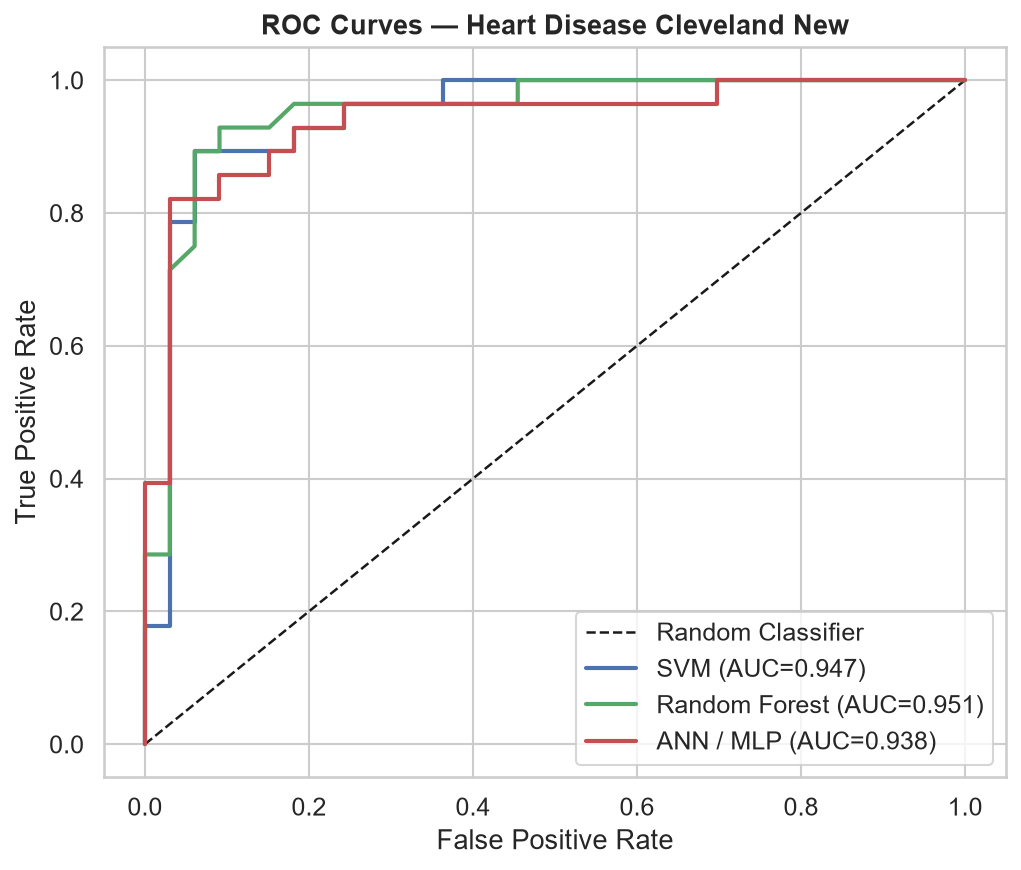
\includegraphics[width=0.72\textwidth]{base_cle_roc.png}
\caption{ROC curves of the baseline models on the Cleveland hold-out split}
\label{fig:base_roc}
\end{figure}

\section{Cooperative GA--PSO with SVM}
\label{sec:coopsvm}
\subsection{Selected configuration}
The full ten-round run on Cleveland took 2346\,s (about 39 minutes). The first round took 287\,s and each later round took 220--245\,s. The selected configuration is:
\begin{itemize}
\item \textbf{Features (8 of 13):} age, sex, cp, fbs, thalach, exang, ca, thal.
\item \textbf{Hyperparameters:} $C = 0.819$, $\gamma = 0.269$ (RBF kernel).
\item \textbf{Fitness:} 0.8068, i.e.\ a mean 10-fold F1 of 0.8468 before the penalty of $8\times 0.005$.
\end{itemize}
The five attributes dropped were trestbps, chol, restecg, oldpeak and slope. Dropping the first three agrees with their weak correlation with the target ($|r|\le 0.17$). Dropping oldpeak ($r=0.43$) and slope ($r=0.34$) is less obvious, but both describe the exercise ST segment and overlap with exang, thalach and thal. Keeping fbs ($r=0.03$) is the least intuitive choice and suggests that the GA's choice among near-equal masks is partly arbitrary, a point examined in Section~\ref{sec:ablation}.

\subsection{Convergence}
Figure~\ref{fig:conv} shows the fitness after each round. In round~1 the GA reached 0.7877 using default SVM hyperparameters. The swarm then tuned $C$ and $\gamma$ on that mask and raised the fitness to 0.8068. From round~2 onward, the GA (now using the tuned hyperparameters) and the swarm both stayed at 0.8068, and neither the mask nor $\boldsymbol{\theta}^{*}$ changed in the remaining nine rounds. An independent repeat of the run gave identical values, which confirms that the result is reproducible under the fixed seed.

\begin{figure}[htpb]
\centering
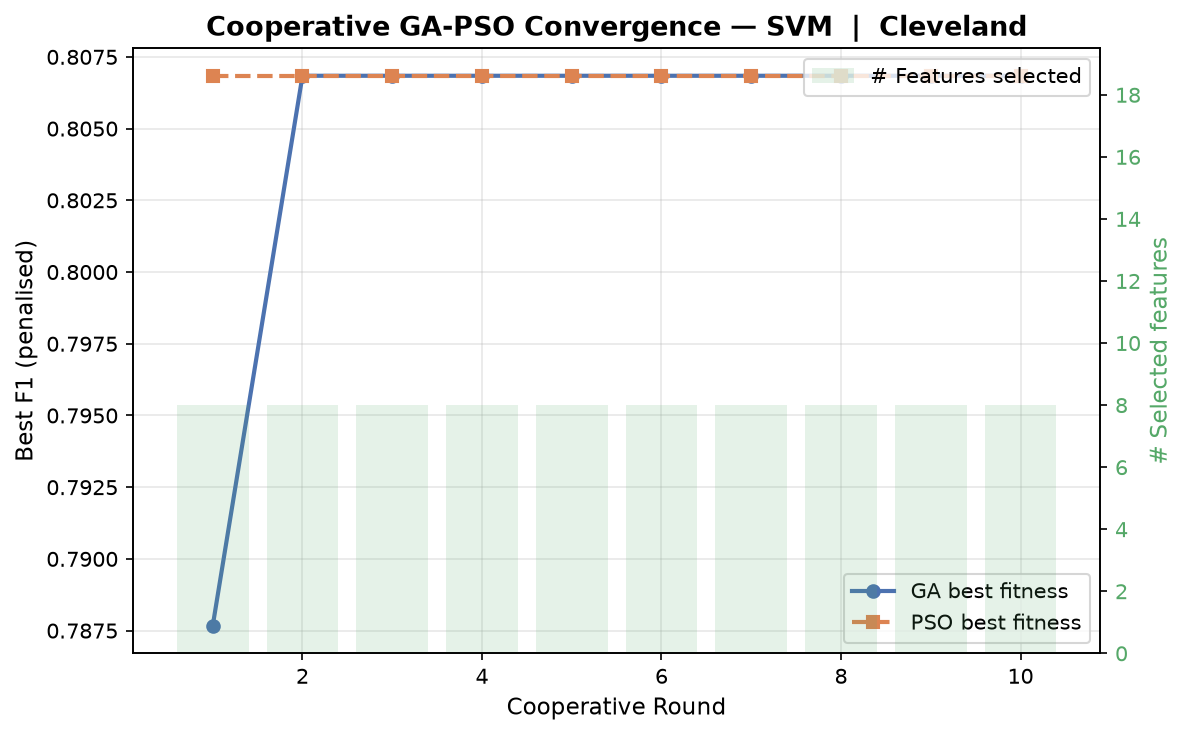
\includegraphics[width=0.78\textwidth]{coop_svm_convergence.png}
\caption{Best fitness per cooperative round for SVM on Cleveland}
\label{fig:conv}
\end{figure}

For the SVM on Cleveland the exchange produced its entire gain in the first round, and the next nine rounds added nothing. The most likely cause is that re-optimizing the mask under the tuned parameters returns the same mask, which is a fixed point of the alternating search. The warm-started, low-inertia swarm then finds nothing better nearby. Whether cooperation helps more on harder settings, such as a classifier with stronger mask--hyperparameter interaction or a larger feature space, is examined by the nested ablation in Section~\ref{sec:ablation}.

\subsection{Out-of-fold performance}
Table~\ref{tab:coop} and Figure~\ref{fig:coop_roc} report the 10-fold out-of-fold evaluation of the selected configuration.

\begin{table}[htpb]
\small
\renewcommand{\arraystretch}{1.25}
\caption{Cooperative GA--PSO (SVM) on Cleveland: 10-fold out-of-fold metrics}
\label{tab:coop}
\begin{tabular}{|p{6cm}|c|}
\hline
\textbf{Metric} & \textbf{Value} \\ \hline
Accuracy & 0.865 \\ \hline
Precision / recall / F1 (macro) & 0.866 / 0.861 / 0.863 \\ \hline
Precision / recall / F1 (weighted) & 0.865 / 0.865 / 0.864 \\ \hline
Disease class: precision / recall & 0.877 / 0.820 \\ \hline
No-disease class: precision / recall & 0.855 / 0.902 \\ \hline
ROC AUC & 0.885 \\ \hline
Average precision & 0.868 \\ \hline
MCC & 0.727 \\ \hline
Confusion matrix (TN, FP, FN, TP) & 148, 16, 25, 114 \\ \hline
Features used & 8 of 13 \\ \hline
\end{tabular}
\end{table}

\begin{figure}[htpb]
\centering
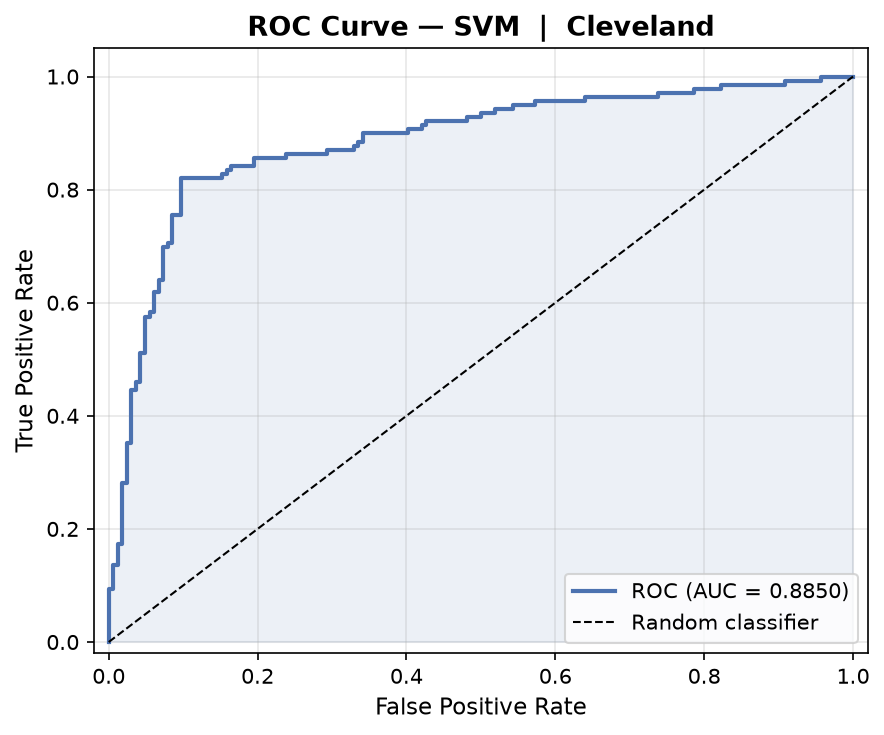
\includegraphics[width=0.6\textwidth]{coop_svm_roc_curve.png}
\caption{ROC curve of the cooperative GA--PSO SVM (out-of-fold)}
\label{fig:coop_roc}
\end{figure}

The tuned 8-feature SVM reaches 0.865 accuracy with an MCC of 0.727. It is more precise on the disease class (0.877) but misses more cases (recall 0.820, 25 false negatives out of 139) than the baselines, which follows from the F1 objective and the lower $C$.

These figures are optimistic, because the folds used to choose the configuration are also used to score it. Section~\ref{sec:ablation} gives the unbiased comparison.

\section{Cooperative GA--PSO with Random Forest (partial)}
A cooperative run for the random forest was stopped after six of ten rounds because each PSO phase took 25--37 minutes. Unlike the SVM, it improved in round~2: the GA found a better 6-feature mask under the tuned forest (fitness 0.7735 to 0.8005) and PSO improved it again to 0.8047 (266 trees, depth 7), after which it plateaued. No XGBoost run was completed.

\section{Nested Cross-Validation Ablation}
\label{sec:ablation}
Table~\ref{tab:ablation} gives the outer-fold test results of the five variants for both settings described in Section~\ref{sec:nested}. Table~\ref{tab:wilcoxon} gives the paired comparisons of the cooperative variant with each of the others, and Figure~\ref{fig:ablation_box} shows the spread over the 15 outer folds.

\begin{table}[htpb]
\small
\renewcommand{\arraystretch}{1.25}
\caption{Nested CV results on Cleveland (mean $\pm$ std over 15 outer test folds)}
\label{tab:ablation}
\begin{tabular}{|p{2.4cm}|c|c|c|c|c|c|}
\hline
\textbf{Variant} & \textbf{Acc.} & \textbf{F1} & \textbf{MCC} & \textbf{AUC} & \textbf{Recall} & \textbf{Features} \\ \hline
\multicolumn{7}{|l|}{\textit{Setting A: $\lambda=0.005$, inner 5-fold CV}} \\ \hline
Baseline    & 0.834$\pm$0.041 & 0.810$\pm$0.051 & 0.666$\pm$0.083 & 0.896 & 0.775 & 13 \\
GA only     & 0.812$\pm$0.053 & 0.789$\pm$0.062 & 0.623$\pm$0.108 & 0.884 & 0.772 & 5.9 \\
PSO only    & \textbf{0.838}$\pm$0.051 & \textbf{0.814}$\pm$0.062 & \textbf{0.676}$\pm$0.104 & \textbf{0.903} & \textbf{0.782} & 13 \\
Sequential  & 0.815$\pm$0.054 & 0.791$\pm$0.065 & 0.630$\pm$0.110 & 0.888 & 0.770 & 5.9 \\
Cooperative & 0.811$\pm$0.058 & 0.784$\pm$0.069 & 0.622$\pm$0.117 & 0.883 & 0.758 & 6.1 \\ \hline
\multicolumn{7}{|l|}{\textit{Setting B: $\lambda=0$, inner 5-fold CV repeated twice}} \\ \hline
Baseline    & 0.834$\pm$0.041 & 0.810$\pm$0.051 & 0.666$\pm$0.083 & 0.896 & 0.775 & 13 \\
GA only     & 0.811$\pm$0.048 & 0.784$\pm$0.058 & 0.620$\pm$0.097 & 0.879 & 0.753 & 8.0 \\
PSO only    & \textbf{0.838}$\pm$0.053 & \textbf{0.813}$\pm$0.064 & \textbf{0.677}$\pm$0.107 & \textbf{0.904} & \textbf{0.775} & 13 \\
Sequential  & 0.806$\pm$0.046 & 0.780$\pm$0.055 & 0.614$\pm$0.092 & 0.883 & 0.753 & 7.9 \\
Cooperative & 0.811$\pm$0.048 & 0.783$\pm$0.057 & 0.622$\pm$0.098 & 0.885 & 0.748 & 7.6 \\ \hline
\end{tabular}
\end{table}

\begin{table}[htpb]
\small
\renewcommand{\arraystretch}{1.25}
\caption{Paired comparison of the cooperative variant with each other variant (accuracy; wins/ties/losses over 15 outer folds and Wilcoxon $p$)}
\label{tab:wilcoxon}
\begin{tabular}{|p{2.6cm}|c|c|c|c|}
\hline
 & \multicolumn{2}{c|}{\textbf{Setting A}} & \multicolumn{2}{c|}{\textbf{Setting B}} \\ \cline{2-5}
\textbf{Cooperative vs.} & \textbf{$\Delta$acc, W/T/L} & \textbf{$p$} & \textbf{$\Delta$acc, W/T/L} & \textbf{$p$} \\ \hline
Baseline   & $-0.023$, 2/2/11 & 0.008 & $-0.023$, 2/1/12 & 0.035 \\ \hline
GA only    & $-0.001$, 3/8/4  & 0.490 & $+0.000$, 5/4/6  & 0.560 \\ \hline
PSO only   & $-0.028$, 0/5/10 & 0.005 & $-0.027$, 3/2/10 & 0.023 \\ \hline
Sequential & $-0.004$, 1/10/4 & 0.136 & $+0.005$, 4/8/3  & 0.498 \\ \hline
\end{tabular}
\end{table}

\begin{figure}[htpb]
\centering
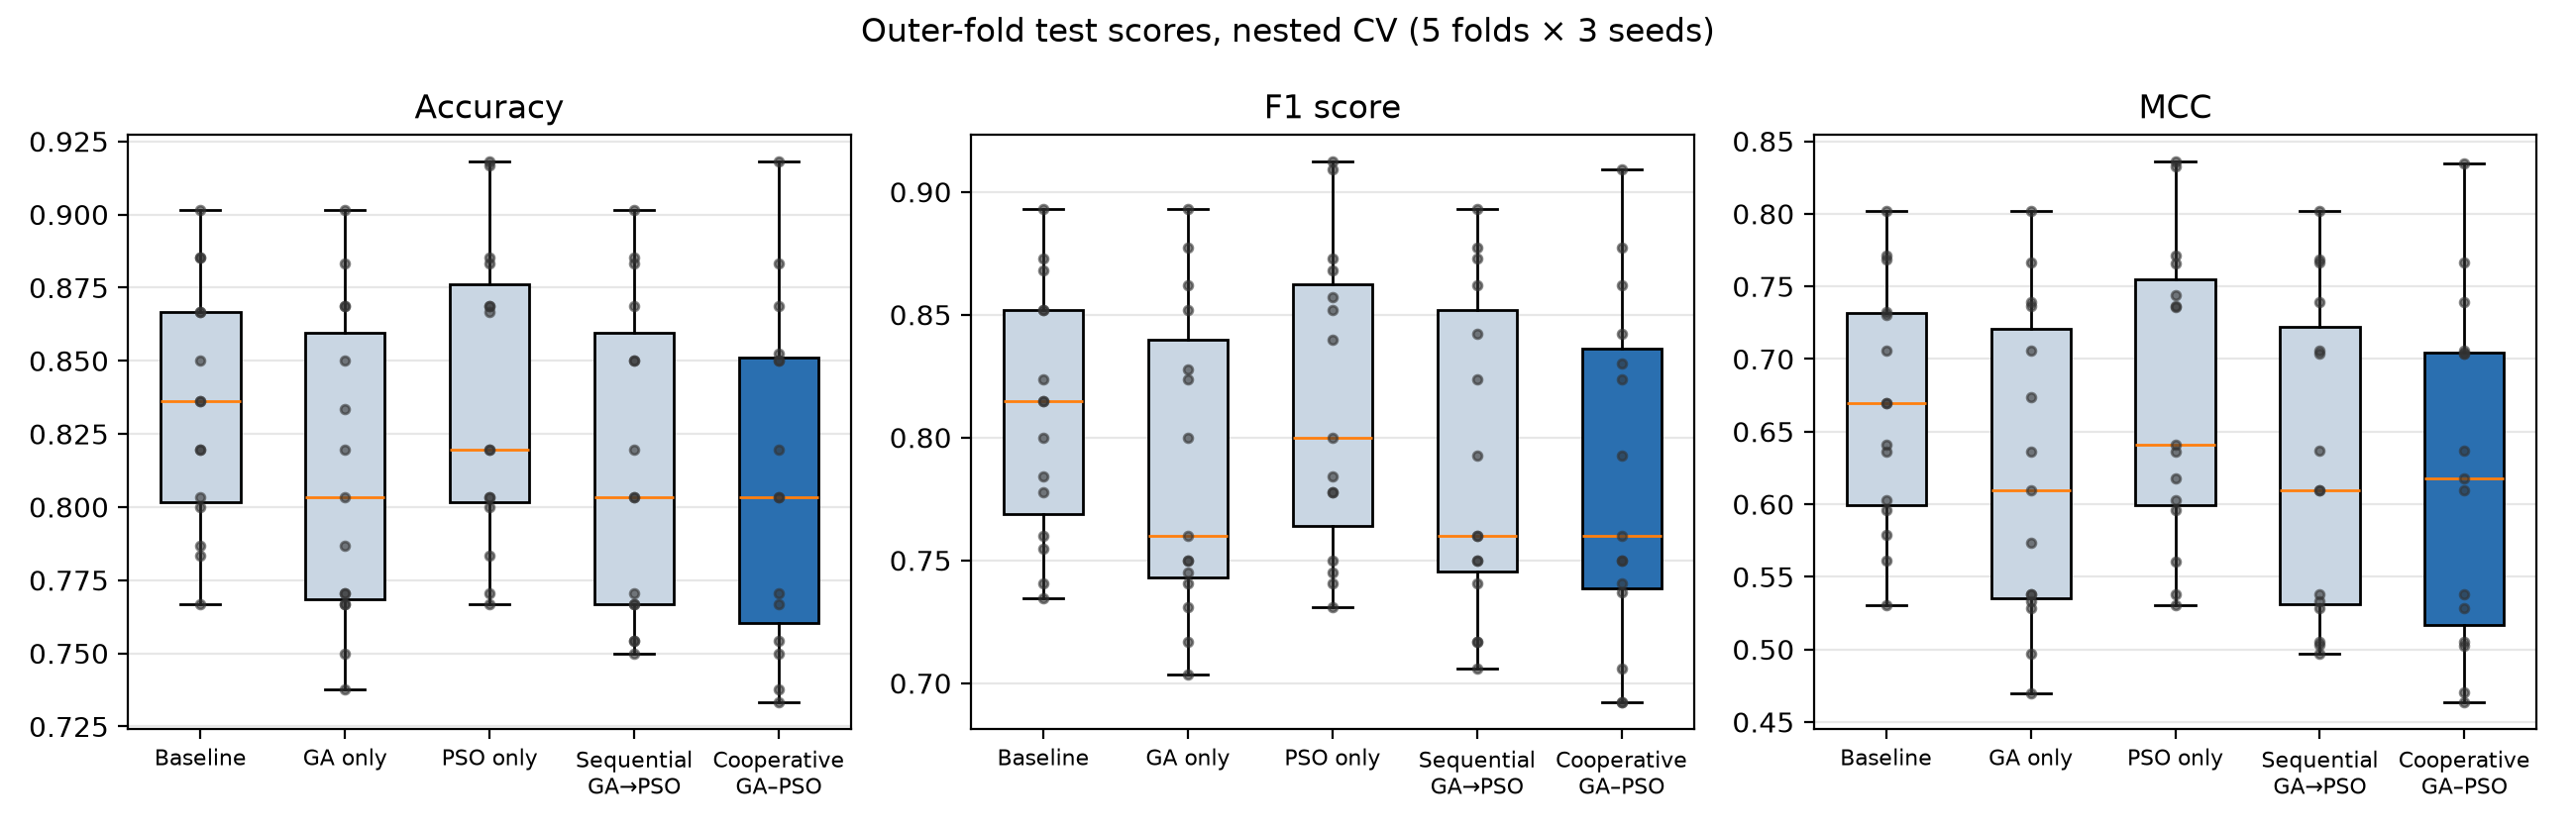
\includegraphics[width=\textwidth]{ablation_boxplot.png}
\caption{Outer-fold test accuracy, F1 and MCC of the five variants (Setting A); each dot is one outer fold}
\label{fig:ablation_box}
\end{figure}

\subsection{What the ablation shows}
\begin{enumerate}
\item \textbf{The cooperation improves the search objective.} Averaged over the 15 outer folds, the best inner fitness of the cooperative variant rose from 0.805 after round~1 to 0.808 after round~2 and 0.808 after round~3. In round~2 the GA, now working with tuned parameters, found better masks than in round~1, which is the two-way benefit the design is meant to provide.
\item \textbf{The improvement does not reach unseen patients.} On the outer folds the cooperative variant is level with the sequential and GA-only variants (no significant difference in either setting). It is significantly worse than PSO-only tuning on all 13 attributes, by about 2.7 points of accuracy and 5 points of MCC, losing in 10 of 15 folds. Removing the feature penalty and doubling the inner folds (Setting~B) changes none of these conclusions.
\item \textbf{Feature selection is the step that overfits.} Every variant that selects features (GA only, sequential, cooperative) lies below the two variants that keep all 13 attributes. With about 242 training patients per outer fold, the difference in inner CV score between good masks is smaller than the noise of the estimate. A wrapper that searches hundreds of masks therefore picks masks that fit the inner folds by chance. Tuning two continuous SVM parameters is a much smaller search and does not show this effect.
\item \textbf{The selected subsets are unstable.} Figure~\ref{fig:ablation_feat} shows how often each attribute was chosen by the cooperative variant across the 15 outer folds. Only \texttt{ca} (15/15) and \texttt{thal} (14/15) were chosen in nearly every fold, followed by \texttt{cp} (12/15). Subset size ranged from 4 to 8, and the tuned $C$ ranged from 0.16 to 786. The subset reported in Section~\ref{sec:coopsvm} (8 attributes) is therefore one of many near-equivalent subsets.
\item \textbf{Budget.} Because masks are cached, the variants that use the GA performed fewer distinct evaluations (about 1000 for cooperative and 940 for sequential) than PSO-only (about 1400). This favours PSO-only somewhat, but GA-only and sequential, with similar budgets, perform the same as cooperative. The budget difference therefore does not explain the gap.
\end{enumerate}

\begin{figure}[htpb]
\centering
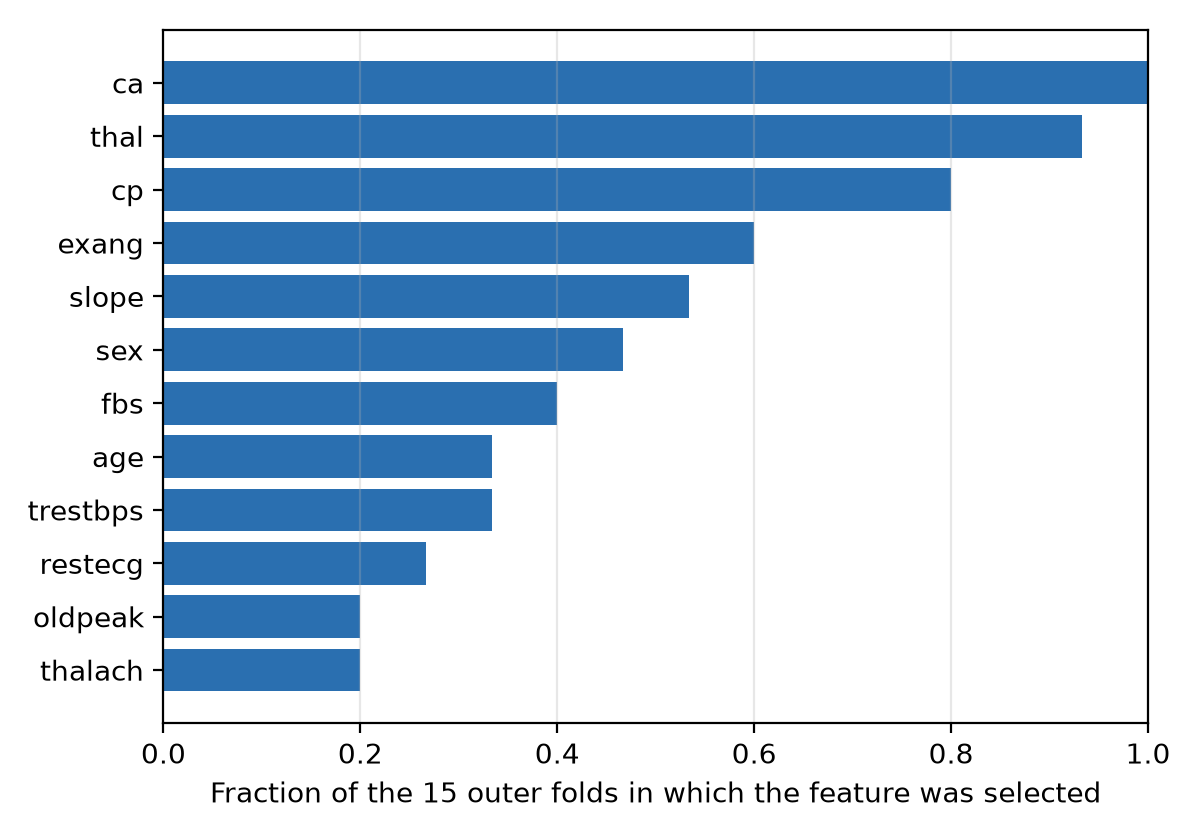
\includegraphics[width=0.7\textwidth]{ablation_feature_stability.png}
\caption{Fraction of outer folds in which each attribute was selected by the cooperative variant (Setting A)}
\label{fig:ablation_feat}
\end{figure}

These results answer the research question in Section~\ref{sec:problem} for the SVM on Cleveland. Repeated GA--PSO exchange finds configurations that score higher on the data used for the search, but not configurations that generalise better than a one-pass pipeline, and neither beats tuning alone. The out-of-fold figures of Section~\ref{sec:coopsvm} (accuracy 0.865) overstate the cooperative SVM by about five points. That gap is the size of the selection bias described by \citet{varma2006bias} and \citet{cawley2010overfitting}.

\section{Overlap between the Statlog and Cleveland Datasets}
\label{sec:overlap}
The project proposal argued that validating on both Cleveland and Statlog would address the single-dataset limitation of prior work. A record-by-record comparison on all 13 attributes shows that this argument does not hold. \textbf{Every one of the 270 Statlog records also appears in the Cleveland file, and all 270 carry the same label.} Statlog is therefore a subset of Cleveland, consisting of 270 of its 303 patients, and not an independent cohort. This is consistent with the near-identical attribute statistics of the two files. For example, both have a mean age of 54.4 and a mean cholesterol close to 247--250\,mg/dl.

Results on Statlog therefore say little about generalisation beyond Cleveland, and a model tuned on Cleveland and tested on Statlog would largely be scored on its own training patients. Independent validation needs a separate source such as the Hungarian, Swiss or VA Long Beach subsets, or the Z-Alizadeh Sani dataset \citep{alizadehsani2013}.

\section{Limitations of the Current Results}
\label{sec:limits}
\begin{itemize}
\item \textbf{Selection bias in the full-data run.} The out-of-fold metrics of Section~\ref{sec:coopsvm} come from the same folds that guided the search. The nested ablation (Section~\ref{sec:ablation}) is the unbiased estimate and should be used for any comparison.
\item \textbf{One classifier in the ablation.} The nested ablation covers the SVM only. The random forest run stopped after six rounds and XGBoost was not run, so the conclusions may not carry over to tree ensembles, whose feature--parameter interaction is stronger.
\item \textbf{One cohort.} All results are on Cleveland. Because Statlog is contained in Cleveland, no independent cohort has yet been tested.
\item \textbf{Shorter schedule in the ablation.} To fit 75 nested searches into the available time, the ablation used 3 rounds with an inner 5-fold CV, against 10 rounds with 10-fold CV in the full run. The full run showed no gain after round~1, so the shorter schedule is unlikely to change the conclusion, but this was not tested.
\item \textbf{Class balancing not applied.} SMOTE \citep{chawla2002smote} was proposed in the first review. With a positive rate of 45.9\%, however, the need for it is modest, and it has not been added. If it is added, it must be applied inside each training fold only.
\item \textbf{Cost.} The RF run shows that the current schedule is too expensive for ensemble models without parallel or early-stopped evaluation.
\end{itemize}

%------------------------------------------------------------------------------------------------%
\chapter{Conclusion and Future Enhancements}
\label{chap:conclusion}

\section{Conclusion}
This thesis built and evaluated a cooperative evolutionary approach to coronary artery disease prediction. A reproducible pipeline loads and validates the data, prevents scaling leakage, and produces untuned SVM, RF and MLP baselines. On Cleveland these reach hold-out accuracies of 0.852--0.885 and cross-validated accuracies of 0.760--0.826. A cooperative GA--PSO optimizer was designed and implemented in which a DEAP genetic algorithm searches feature masks and a PySwarms swarm searches classifier hyperparameters, and the two exchange their best solutions every round under a shared, penalised 10-fold F1 objective.

For the SVM, the optimizer reduced the input to eight attributes (age, sex, chest-pain type, fasting blood sugar, maximum heart rate, exercise angina, number of vessels and thallium result). It reached an out-of-fold accuracy of 0.865, macro F1 of 0.863 and MCC of 0.727, and the result was reproducible across runs.

The central experiment of the thesis is the nested cross-validation ablation, which compared the cooperative scheme with an untuned baseline and with GA-only, PSO-only and sequential variants on the same 15 outer folds. Its findings are:
\begin{enumerate}
\item The two-way exchange works as a search method: the GA found better masks once it received tuned parameters, and the inner fitness rose in each round.
\item On unseen patients, the cooperative SVM (accuracy 0.811, MCC 0.622) is no better than the sequential or GA-only variants, and is significantly worse than tuning the SVM on all 13 attributes (accuracy 0.838, MCC 0.676). The result holds with and without the feature penalty and with repeated inner folds.
\item Wrapper feature selection is the source of the loss. At about 240 training patients it overfits the inner folds, and the chosen subsets are unstable. Only the number of major vessels and the thallium result are selected consistently.
\item The full-data out-of-fold estimate overstates the cooperative SVM by about five points of accuracy, which shows how large selection bias can be at this sample size.
\item All 270 Statlog records are contained in Cleveland. Studies that treat the two as independent or pool them may report inflated results.
\end{enumerate}
The practical conclusion is that, for small CAD datasets, a hybrid evolutionary scheme should be judged by nested, ablated evaluation and not by the score of its own search. On this dataset the better model is the simpler one, PSO tuning on all attributes. The cooperative GA--PSO design is likely to pay off only where the fitness estimate is reliable enough for subset differences to generalise: on larger cohorts, with more candidate features, or with a stability-aware fitness.

\section{Future Enhancements}
The following extensions follow directly from these findings:
\begin{enumerate}
\item \textbf{Stability-aware fitness.} Score masks by their mean and variance over repeated inner CV, or by how often they agree across bootstrap samples, so that the GA prefers subsets that are stable rather than lucky.
\item \textbf{Larger and independent cohorts.} Repeat the ablation on the Z-Alizadeh Sani dataset \citep{alizadehsani2013}, which has 54 attributes, and on the Hungarian, Swiss and VA Long Beach data, where feature selection has more room to help. The model tuned on Cleveland should also be tested on these without retuning.
\item \textbf{Clinically weighted objectives.} Compare F1 with F$_2$ and recall-at-fixed-specificity objectives, and tune the decision threshold.
\item \textbf{Interpretability.} Add SHAP explanations \citep{lundberg2017shap} for the final models, both global attribute importance and per-patient explanations, and check that they agree with the GA's feature choices.
\end{enumerate}

%------------------------------------------------------------------------------------------------%
\begin{singlespace}
  \bibliography{thesis_refer}
\end{singlespace}
\addcontentsline{toc}{chapter}{REFERENCES}
\appendix

\begin{appendices}
\chapter*{APPENDIX}
\section*{A. Reproducing the Experiments}
\begin{verbatim}
python -m venv venv
.\venv\Scripts\Activate.ps1
pip install -r requirements.txt
python -m src.baseline_models
python -m src.cooperative_ga_pso --dataset cleveland --classifier SVM
python -m src.evaluate_hybrid --result all
pytest
\end{verbatim}

\section*{B. Reproducing the Nested Ablation}
\begin{verbatim}
python -m src.ablation_nested                      # Setting A
$env:ABL_TAG="_lambda0_rep2"; $env:ABL_LAMBDA="0"; $env:ABL_REPEATS="2"
python -m src.ablation_nested                      # Setting B
python -m src.plot_ablation
\end{verbatim}
Setting~A took 751\,s and Setting~B 1487\,s on an 8-core desktop. Raw per-fold results, summaries and test statistics are written to \texttt{results/ablation/} and \texttt{results/ablation\_lambda0\_rep2/}.
\end{appendices}
%%%%%%%%%%%%%%%%%%%%%%%%%%%%%%%%%%%%%%%%%%%%%%%%%%%%%%%%%%%%
\end{document}
